\chapter{Network Architectures and Training Processes} % Main chapter title

\label{Chapter 3} % Change X to a consecutive number; for referencing this chapter elsewhere, use \ref{ChapterX}  

We compared three network architectures, each in two different sizes, and evaluated them on a handwritten digit recognition task. The first architecture, which we called PanNet, was a stacked convolutional autoencoder trained layerwise with a fully connected classification layer on top. The second architecture was our implementation of a well-known conventionally rained CNN, LeNet. The third network, BackPanNet, had the same architecture as PanNet but had a round of backpropagation training across the whole network after initial autoencoder training.

Network architectures are summarized in figure \ref{fig:network architecture} and table \ref{tab:summary}. 


%----------------------------------------------------------------------------------------
%	SECTION 1
%----------------------------------------------------------------------------------------

%-----------------------------------
%	SECTION 2
%-----------------------------------
\section{Network Architectures}

\subsection{PanNet and BackPanNet}

All networks in this work were implemented using TensorFlow [cite].

PanNet consists of X layers. The first layer, C1, is XxX. The second layer has X filters, each XxX pixels wide. The first pooling layer P1 is .... etc. [just start with a very simple paragraph describing the exact architecture. Probably a good idea to add names for the layers, you can put these in the figures, for clarity. You could call them C1, P1, C2, P2, L1, as I've done here, or maybe it's better C1,P2,C3,P4,L5 for the convolutional, pooling, and final classification layers.] The final classification layer, L1, had X units.

PanNetEnlarged has the same structure, except that layers 2 and 3 have X and Y filters, respectively.

L1 units were activated according to pixel values of individual  images from the training set.

To compute the activation in C2, the C1 activations are first zero-padded. The C2 activation is then given by [put convolution formula in here], with the ReLU activation function [put formula here].

The activation in the P1 was computed according to [put formula in here].

Activations in C3 and P2 were computed analogously [is this true?].

Activations in L1 were computed according to [put formula here]

BackPanNet and BackPanNet-enlarged share the same architecture, although with different training, as we will describe shortly.

\subsection{LeNet}

To compare BackPan's performance with a well-known CNN, we implemented a version of LeCun's 1998 network LeNet \cite{lecun_gradient-based_1998}, with several small changes.

[Here describe the network in very similar language to that used for PanNet. You can copy and paste and then make the required changes.]

We also created an enlarged version of LeNet, to compare with our PanNet-enlarged. LeNet-enlarged had X filters in layer Y, etc.

Our version of LeNet differed from the original in three [or however many] ways: first, we used ReLU units instead of logistical units. Second, something about the padding (was this in fact different?) Third, our training procedure differed slightly, as we will describe.



\begin{figure}[th]
\centering
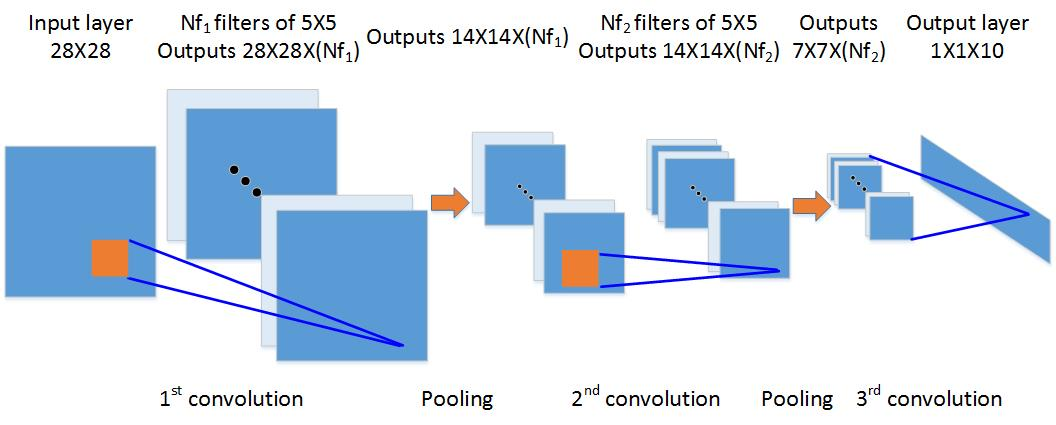
\includegraphics[width=140mm]{Figures/Network_Architecture}
\decoRule
\caption{[Replace all this with a simple description of what you are seeing. Label the figure with the names of the layers.]
Network architectures: all networks adopt the convolutional neural network architecture. PanNet(-enlarged) and backPanNet(-enlarged) use same padding algorithm but LeNet-1(-enlarged) uses valid padding algorithm, which means no padding. As a result, the outputs of LeNet-1(-enlarged) from \(1^{st}\) and \(2^{nd}\) convolution are of dimension \(24 \times 24\) and \(8 \times 8\) respectively instead. Pooling algorithm is \(2 \times 2\) max-pooling. Number of filters for the first convolutional layer \(Nf_{1}\) and the one for the second convolutional layer \(Nf_{2}\) are (4, 12) for regular networks and (120, 150) for enlarged networks. }
\label{fig:network architecture}
\end{figure}



%-----------------------------------
%	SECTION 3
%-----------------------------------

\section{Training}

\subsection{Training data}

We trained our networks using the well-known database of 28x28 pixel handwritten digits, MNIST \cite{noauthor_mnist_nodate}. The dataset consists of 55,000 training images, with 5,000 more in validation set and 10,000 in a testing set.

\begin{figure}[th]
\centering
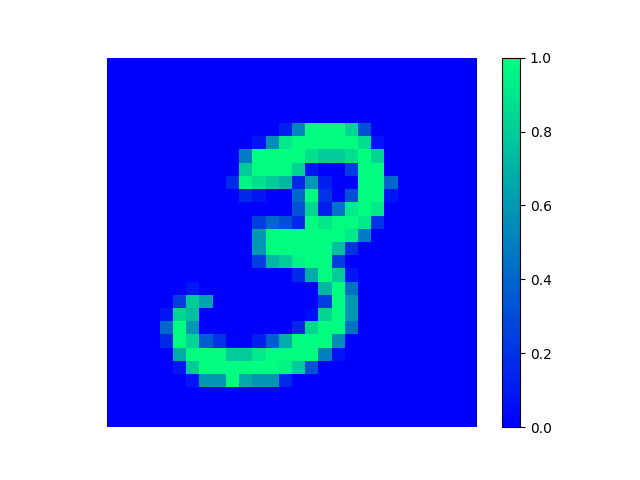
\includegraphics[width=50mm]{Figures/Input}
\decoRule
\caption{A sample MNIST image: MNIST images have a height and width of 28 pixels with each pixel indicating the gray level. The value of each pixel is between 0 and 1.}
\label{fig:input}
\end{figure}

\subsection{Training algorithms}


\subsubsection{PanNet and PanNet-enlarged}

PanNet was trained layerwise in three steps. In the first step (Figure X, orange box), the connections from C1 to C2 were trained using the [name it] algorithm with minibatches of 100 images, to minimize the convolutional autoencoder loss function: [give formula here]. We determined that this loss function was appropriately minimized after X images [reference figure here]. Therefore we halted training and froze the C1 to C2 (or whatever) weights after X training images.

In the second step (Figure X, green box), training images were fed through the fixed network to determine C2 activations. Then the C2 - C3 connections were trained analogously to the previous layer. We halted training after X images (reference figure here).

In the third step (Figure X, purple box), the classification layer was trained using X algorithm to minimize the loss function [put formula here]. We trained for X images.

The learning rates for the three steps were chosen to maximize final accuracy (show figure) and were set to be 0.1, 0.1, and 0.3 (or whatever), respectively.

PanNet-enlarged was trained in a similar manner, except [put in any differences here]


\subsubsection{LeNet}

[Describe LeNet training in similar fashion to what I put above. At the end, put a paragraph noting any differences to the original paper, with a few words about why you made that choice.]

LeNet-enlarged was trained analogously.

\begin{figure}[th]
\centering
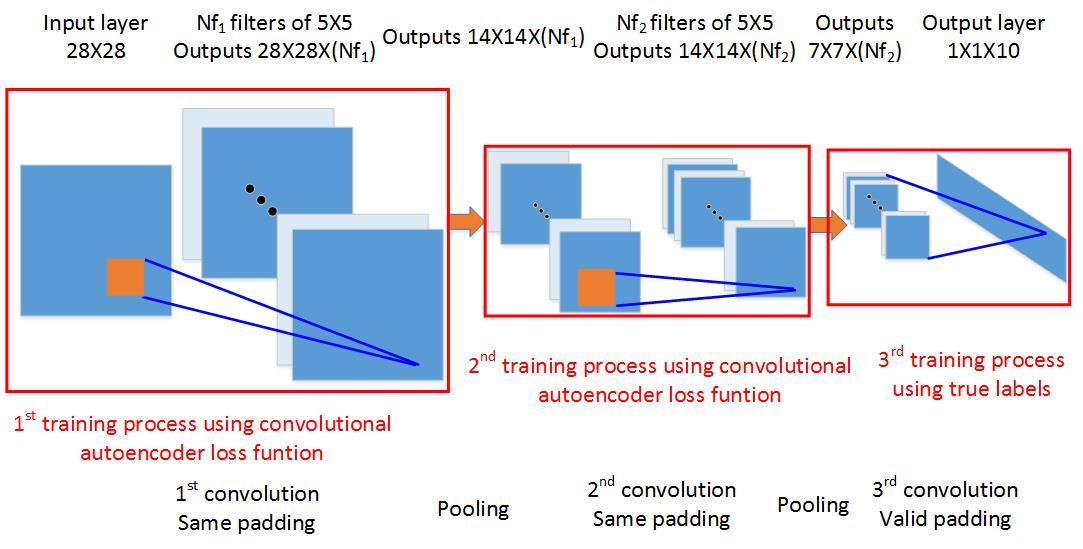
\includegraphics[width=140mm]{Figures/PanNet-training}
\decoRule
\caption{Training process for PanNet(-enlarged): the first convolutional layer is firstly trained aiming to minimize autoencoder loss function, with the goal to reproduce the input information. Weights and biases for the first convolutional layer are fixed after the first training process. Then the second convolutional layer is trained using autoencoder loss function, with the goal to reproduce information entering the second convolutional layer. Weight and biases for the second convolutional layer are fixed after the second training process. Finally, the third layer is trained with cross entropy loss function using the true labels.}
\label{fig:PanNet-training}
\end{figure}

\subsubsection{BackPanNet}

BackPanNet had the same training procedure as PanNet, with the addition of a fourth step (Figure X). In this step, conventional backpropagation was used to modify all the weights in the network using the [name it] algorithm to minimize the loss function [give the formula or say it's the same as for PanNet]. This fourth training step was trained for X images.

BackPanNet-enlarged was trained analogously.

\begin{figure}[th]
\centering
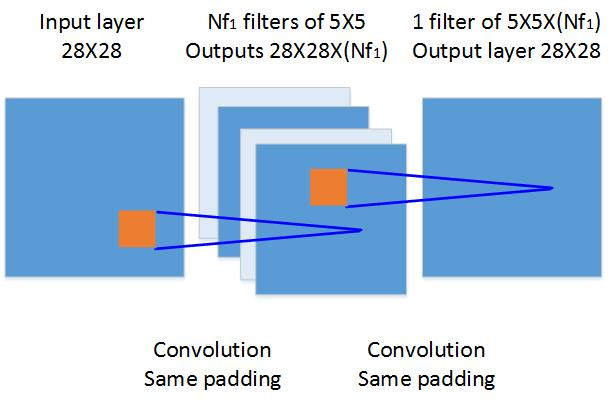
\includegraphics[width=60mm]{Figures/PanNet_first_training}
\decoRule
\caption{Training process for PanNet(-enlarged) - the first training step: this network is trained aiming to enable outputs reproduce inputs. After the first training step, encoder weights and biases are used in the original network.}
\label{fig:PanNet_first_training}
\end{figure}
\subsection{Training Process for LeNet-1 and LeNet-1-enlarged}


\begin{figure}[th]
\centering
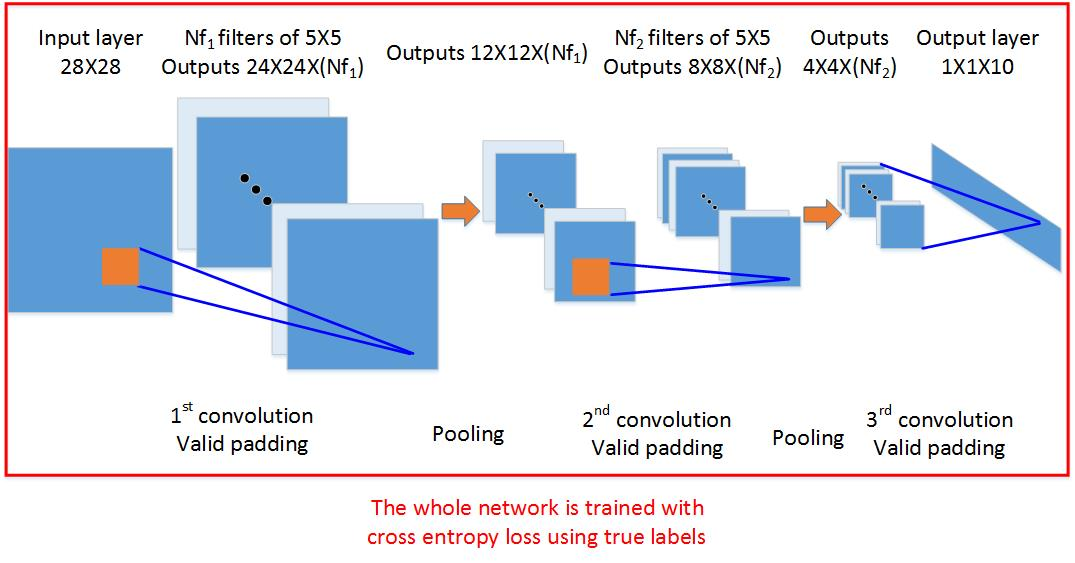
\includegraphics[width=140mm]{Figures/LeNet-1-training}
\decoRule
\caption{Training Process for LeNet-1(-enlarged)}
\label{fig:LeNet-1-training}
\end{figure}

\subsection{Training Process for backPanNet and backPanNet-enlarged}


\begin{figure}[th]
\centering
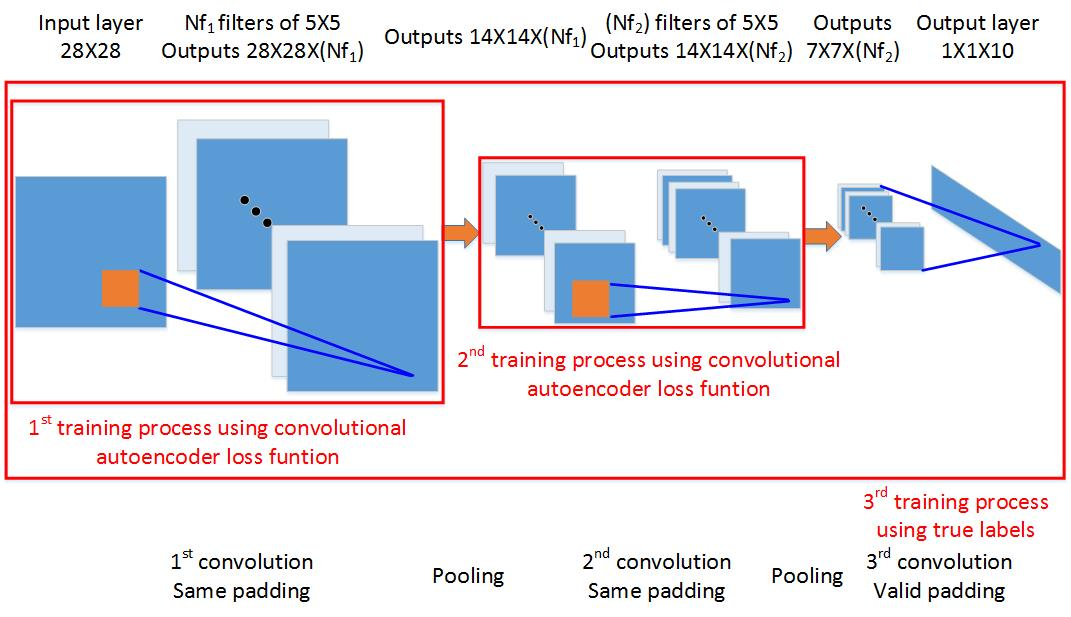
\includegraphics[width=140mm]{Figures/backPanNet-training}
\decoRule
\caption{Training Process for backPanNet(-enlarged): Firstly, backPanNet(-enlarged) is trained using autoencoder loss functions for the first two convolutional layers. Weights and biases of the first convolutional layer are pre-fixed during the training step for the second convolutional layer. Using the results from stacked convolutional autoencoder training process as initial values for the first two convolutional layers, the network is then trained using cross entropy with true labels and error backpropagation among the whole network.}
\label{fig:backPanNet-training}
\end{figure}

%----------------------------------------------------------------------------------------
%	SECTION 4
%----------------------------------------------------------------------------------------
\section{Hyperparameter Selection}

\subsection{Hyperparameter Selection for PanNet} 


[I'm not sure you need this section in the end. Perhaps move this info to the figure captions and just have the figures, something like "Autoencoder loss as a function of training number, calculated using validation set. The loss is appropriately minimized after [X] images. ] 

Firstly, learning rates are fixed to be 0.1 for all training steps based on experience. These relatively large learning rates help improving training efficiency. Absence of oscillation in penalty versus number of training batches plots can reassure the learning rates selection.  




The first convolutional layer of PanNet is initially trained with 10,000 batches. Loss function is calculated using validation set after first batch and every another 250 batches before 10,000 batches. Penalty versus number of training batches plot is shown in figure \ref{fig:PanNet_search_parameters_1}. As can be seen from the plot, loss function flattens out after 4,000 batches, so the number of training batches for the first layer of PanNet is chosen to be 4,000. 

\begin{figure}[th]
\centering
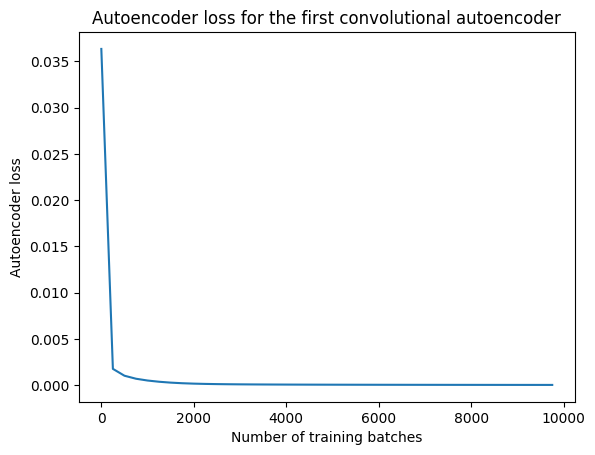
\includegraphics[width=60mm]{Figures/PanNet_search_parameters_1}
\decoRule
\caption{PanNet\\ First autoencoder loss versus number of training batches}
\label{fig:PanNet_search_parameters_1}
\end{figure}

After the first layer is trained with 4,000 batches, the second convolutional layer is trained with 10,000 batches. Loss function is calculated using validation set after the first batch and every another 250 batches before 10,000 batches. Penalty versus number of training batches plot is shown in figure \ref{fig:PanNet_search_parameters_2}. As can be seen from the plot, the loss function flattens out after 6,000 batches, so the number of training batches for the second layer of PanNet is chosen to be 6,000. 

\begin{figure}[th]
\centering
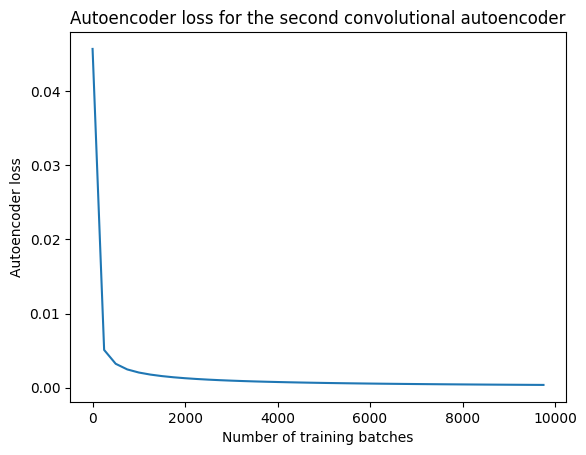
\includegraphics[width=60mm]{Figures/PanNet_search_parameters_2}
\decoRule
\caption{PanNet\\ Second autoencoder loss versus number of training batches}
\label{fig:PanNet_search_parameters_2}
\end{figure}

After the first layer is trained with 4,000 batches and the second layer is trained with 6,000 batches, the final layer is trained with 50,000 batches using cross entropy loss function. Cross entropy loss is calculated every 1,000 batches using validation set. Penalty and accuracy versus number of training batches plots are shown in figure \ref{fig:PanNet_search_parameters_3}. As can be seen from the plot, the loss function keeps decreasing until 50,000 batches, so the number of training for the third layer of PanNet is studied until 50,000 batches.  

\begin{figure}[th]
\centering
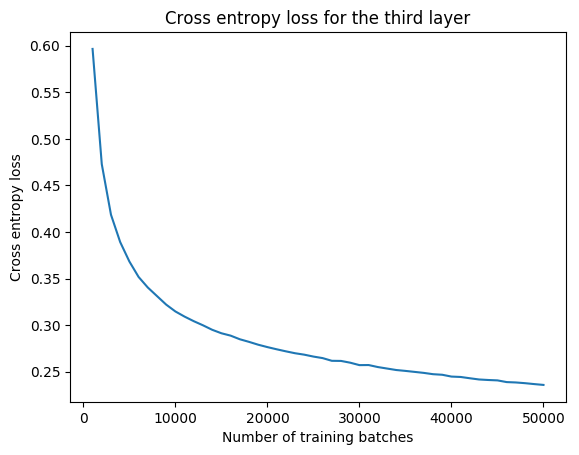
\includegraphics[width=60mm]{Figures/PanNet_search_parameters_3_loss}
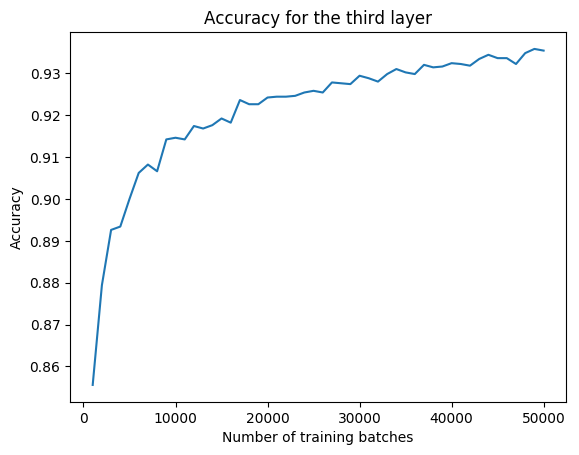
\includegraphics[width=60mm]{Figures/PanNet_search_parameters_3_accuracy}
\decoRule
\caption{PanNet\\ Final cross entropy loss and accuracy versus number of training batches}
\label{fig:PanNet_search_parameters_3}
\end{figure}

\subsection{Hyperparameter Selection for PanNet-enlarged}

Following the exactly same procedure, numbers of training batches for each layer of PanNet-enlarged are determined. The learning rates are also fixed to be 0.1 for all training steps. Plots associated with hyperparameter selection of PanNet-enlarged are shown in figure \ref{fig:PanNet-enlarge_selection}. As a result, the first convolutional layer of PanNet-enlarged will be trained with 2,000 batches, next second layer with 2,000 batches and then third layer with 50,000 batches. 

\begin{figure}[th]
\centering
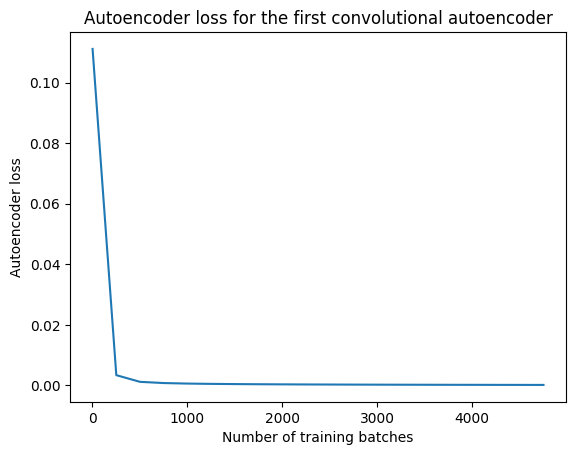
\includegraphics[width=60mm]{Figures/PanNet-enlarged_search_parameters_1}
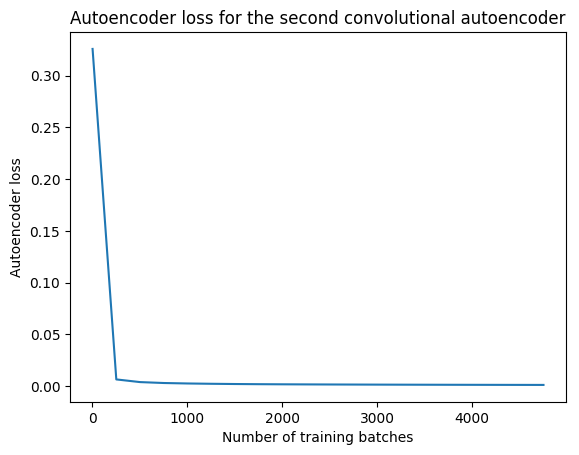
\includegraphics[width=60mm]{Figures/PanNet-enlarged_search_parameters_2}
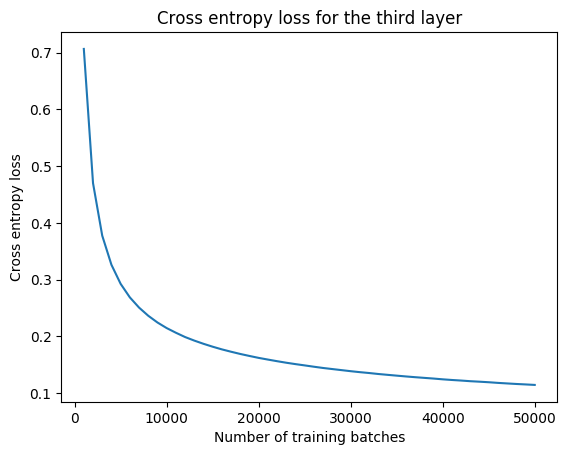
\includegraphics[width=60mm]{Figures/PanNet-enlarged_search_parameters_3_loss}
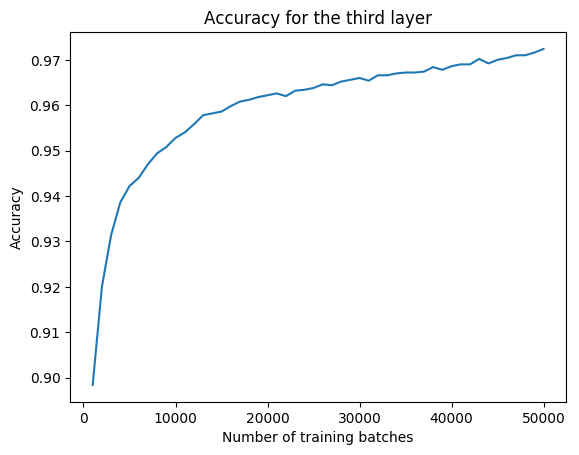
\includegraphics[width=60mm]{Figures/PanNet-enlarged_search_parameters_3_accuracy}
\decoRule
\caption{Hyperparameter Selection for PanNet-enlarged}
\label{fig:PanNet-enlarge_selection}
\end{figure}

%----------------------------------------------------------------------------------------
%	SECTION 5
%----------------------------------------------------------------------------------------
\section{Summary}

\begin{sidewaystable}
\centering
\caption{Summary of all neural networks}\label{tab:summary}
\begin{tabular}{l c c c c c c}
\toprule
& PanNet & \makecell{PanNet\\-enlarged}& LeNet-1 & \makecell{LeNet-1\\-enlarged}  & backPanNet & \makecell{backPanNet\\-enlarged}\\
\midrule
\makecell[l]{Number of filters\\in first layer} & 4 & 120 & 4 & 120 & 4 & 120\\
\makecell[l]{Dimension of filters\\in first layer}  & [5, 5] & [5, 5] & [5, 5] & [5, 5] & [5, 5] & [5, 5]\\
\makecell[l]{Activation function\\in first layer} & Relu & Relu & Relu & Relu & Relu & Relu\\
\makecell[l]{Number of filters\\in second layer} & 12 & 150 & 12 & 150 & 12 & 150\\
\makecell[l]{Dimension of filters\\in second layer}  & [5, 5] & [5, 5] & [5, 5] & [5, 5] & [5, 5] & [5, 5]\\
\makecell[l]{Activation function\\in second layer} & Relu & Relu & Relu & Relu & Relu & Relu\\
\makecell[l]{Activation function\\in third layer} & softmax & softmax & softmax & softmax & softmax & softmax\\
\makecell[l]{Standard deviation\\ of weight initialization} & 0.1 & 0.1 & 0.1 & 0.1 & 0.1 & 0.1\\
\makecell[l]{Padding\\for convolutions} & \makecell{Same\\Valid for final\\layer} & \makecell{Same\\Valid for final\\ layer} & Valid & Valid  & \makecell{Same\\Valid for final\\ layer} & \makecell{Same\\Valid for final\\ layer}\\
Learning rate & [0.1, 0.1, 0.1] & [0.1, 0.1, 0.1] & 0.1 & 0.1  & [0.1, 0.1, 0.1] & [0.1, 0.1, 0.1]\\
Batch size & 100 & 100 & 100 & 100 & 100 & 100\\
Number of training batches & \makecell{[4000, 6000\\, 50000]} & \makecell{[2000, 2000\\, 50000]} & 50,000 & 50,000 & \makecell{[4000, 6000\\, 50000]} & \makecell{[2000, 2000\\, 50000]}\\
\bottomrule\\
\end{tabular}
\end{sidewaystable}
